\documentclass{article}
\usepackage[scale=.7]{geometry}
\thispagestyle{empty}
\usepackage{tikz}

\usetikzlibrary{arrows.meta}

\tikzset{
  pics/axes/.style args={#1:#2;#3:#4}{
    code = {
      \draw[help lines,gray] (#1-.5,#3-.5) grid (#2+.5,#4+.5);
      \draw[->,thick] (#1 - .5,0) -- (#2 + .5,0);
      \draw[->,thick] (0,#3 - .5) -- (0,#4 + .5);
      \foreach \x in {#1,...,#2} {
        \ifnum\x=0\else
        \draw[thick] (\x,0) -- (\x,-.2);
        \node[below left] at (\x cm+1ex,-.2) {\(\x\)};
        \fi
      }
      \node[below] at (#2+.5,-.2) {\(x\)};
      \foreach \y in {#3,...,#4} {
        \ifnum\y=0\else
        \draw[thick] (0,\y) -- (-.2,\y);
        \node[below left] at (-.1,\y cm + 1ex) {\(\y\)};
        \fi
      }
      \node[left] at (-.1,#4+.5) {\(y\)};
      \node[below left] at (0,0) {0};
    }
  },
  pics/axes/.default={-6:6;-6:6},
}

\begin{document}
\centering
{\huge \textbf{Find the Area of the Christmas Tree}}

\vspace{1cm}

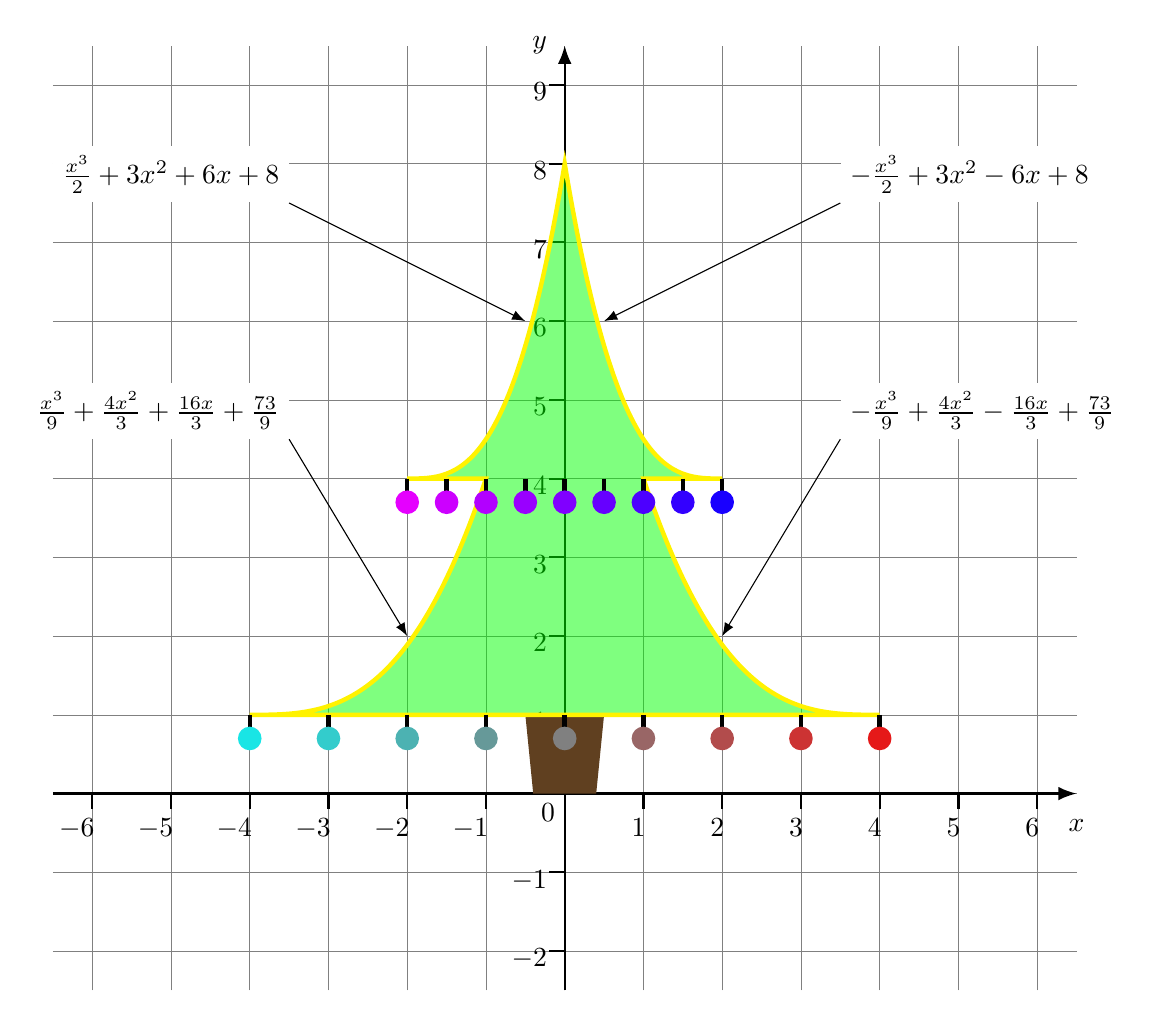
\begin{tikzpicture}[>=Latex]
\pic{axes={-6:6;-2:9}};
\fill[brown!50!black] (-.5,1) -- (-.4,0) -- (.4,0) -- (.5,1);
\filldraw[fill=green,ultra thick,draw=yellow,fill opacity=.5] (-4,1) .. controls +(1,0) and +(-1,-3) .. (-1,4) -- ++(-1,0) .. controls +(2/3,0) and +(-2/3,-4) .. ++(2,4) .. controls +(2/3,-4) and +(-2/3,0) .. ++(2,-4) -- ++(-1,0) .. controls +(1,-3) and +(-1,0) .. ++(3,-3) -- cycle;
\foreach[evaluate=\k as \tint using {(\k+4)*10 + 10}] \k in {-4,...,4} {
  \draw[ultra thick] (\k,1) -- +(0,-.4);
  \fill[red!\tint!cyan] (\k,.7) circle[radius=.15];
  \draw[ultra thick] (\k/2,4) -- +(0,-.4);
  \fill[blue!\tint!magenta] (\k/2,3.7) circle[radius=.15];
}
\draw[<-] (-2,2) -- ++(-1.5,2.5) node[above left,fill=white] {\(\frac{x^3}{9} + \frac{4 x^2}{3} + \frac{16 x}{3} + \frac{73}{9}\)};
\draw[<-] (2,2) -- ++(1.5,2.5) node[above right,fill=white] {\(-\frac{x^3}{9} + \frac{4 x^2}{3} - \frac{16 x}{3} + \frac{73}{9}\)};
\draw[<-] (-.5,6) -- ++(-3,1.5) node[above left,fill=white] {\(\frac{x^3}{2} + 3 x^2 + 6 x + 8\)};
\draw[<-] (.5,6) -- ++(3,1.5) node[above right,fill=white] {\(-\frac{x^3}{2} + 3 x^2 - 6 x + 8\)};
\end{tikzpicture}
\end{document}
